\documentclass[letterpaper,12pt]{article}
\usepackage[utf8]{inputenc}
\usepackage{fullpage}
\usepackage{courier}
\usepackage[margin=0.75in]{geometry}
\usepackage{listings}
\usepackage{color}
\usepackage{graphicx}
\usepackage[width=5in]{caption}
\usepackage{hyphenat}
\usepackage{hyperref}
\usepackage{float}
\usepackage{multirow}

% Format a sectionless paragraph
\newcommand*\unparagraph{
	\par
	\nopagebreak
	\vskip3.25ex plus1ex minus.2ex
	\noindent
}

% define extra colors
\definecolor{dkgreen}{rgb}{0,0.6,0}
\definecolor{purple}{RGB}{159,0,197}

% define the code listing format
\lstset{
	language=C++,
	basicstyle=\footnotesize\ttfamily,
	backgroundcolor=\color{white},
	showspaces=false,
	showstringspaces=false,
	frame=none,
	tabsize=3,
	keywordstyle=\color{purple},
	commentstyle=\color{dkgreen},
	stringstyle=\color{blue},
	escapeinside={\%*}{*)}
}

% efine the title/header
\title{\Large CS 3468\\Lab 5} 
\author{Jared Wallace}
\date{}

\begin{document}

\maketitle

\vspace{30mm}

\section*{Objectives}
\begin{enumerate}
\item Build a sensor application that detects and locates mobile object
\item Understand the pro's and con's of teamwork
\end{enumerate}

\section*{Overview}
In this project, y'all will build a sensor network to track a mobile object
that carries a light. In the network, sensors will detect the object by sensing
the light. Because each sensor has a different distance to the light, the light
intensity recorded by each sensor will vary according to the distance from the source.
By collecting and analyzing all sensing data, the network will be able to detect and
locate the mobile object.

The network will look like the diagram below, where the triangle symbol represents the source
light, the circle symbols represent sensors and the square symbol represents the base station.
The base station will be what collects the data from the sensors and computes the location of
the source light.

Because the network area is large, sensors farther away from the base station will be unable to
communicate directly with the base station. Instead, their data must traverse other sensors in
order to reach the base station. The dashed lines represent how that data is forwarded through
other sensors to reach the base station.
\begin{figure}[H]
	\centering
	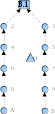
\includegraphics[width=.75in]{network.png}
\end{figure}

\section*{Team}
This will be a whole class effort. Each student will have the responsibility of programming their
own sensor. You will be provided one local base station app for debugging purposes. When we build
the final network, one bad sensor node will break the network (there's the con of teamwork).

I will give you the following information:
\begin{itemize}
    \item The ID of the sensor
    \item The ID of the local base station (your personal debugging base station)
    \item The ID of the next hop
    \item The ID of the previous hop
\end{itemize}

\section*{Tasks}
Implementation of the network takes two steps. First, each student will make a
local application to ensure the sensor can correctly detect light and transmit
data. Then, all sensors will be connected to form a tracking network with a static route.

\subsection*{Part 1}
Create an application that can:
\begin{enumerate}
    \item Sense light every two seconds
    \item Calculate and transmit the average of every three data points and transmit
        that data to the base station (that's once every six seconds for the mathematically
        challenged)
    \item Utilize the LED's to signal the status of the sensor (green for sampling,
        red for transmitting)
\end{enumerate}

\subsection*{Packet Structure}
Also defined in sense.h, the structure is as follows:
\begin{enumerate}
    \item sender\_id: the ID of the sensor that originates the DATA packet, 2 bytes.
    \item cnt: the sequence number, 2 bytes. The sequence number is generated by the
        originating sensor and is incremented for each new DATA packet.
    \item val: the light intensity, 2 bytes.
    \item fwd\_id: the ID of the sensor who is forwarding the DATA packet packet, 2 bytes.
    \item rec\_id: the ID of the base station, 2 bytes.
\end{enumerate}

\subsection*{Part 2}
Implement the tracking network as follows: (network will use a static route, as discussed)
\begin{enumerate}
    \item Sense light every 2 seconds,
    \item Send the average of three data points to the next hop every 6 seconds in a DATA packet.
    \item Use LEDs to indicate the status of the sensors.
    \item Forward the received DATA packets from the previous hop to the next hop.
\end{enumerate}

Your design and implementation should have the following structure:
\begin{enumerate}
    \item The application should have two separate modules: sensing and forwarding.
       The two modules should be in two different .nc files.
    \item The sensing module should indicate if a new data item is generated and sent.
    \item The forwarding module should indicate when a new packet is received and forwarded.
    \item If the transmission fails, the forwarding module should either buffer or discard
       outgoing packets. It's your choice which behavior to implement.
\end{enumerate}


\section*{Lab Report}
\begin{enumerate}
   \item Please demonstrate your program to the lab instructor and let him check your code at the end of the current lab project.
   \item Your project report is due at the beginning of the next lab.
   \item Grading criteria
      \begin{itemize}
         \item Demonstration, 15 percent
         \item Code, 15 percent
         \item Report, 70 percent
      \end{itemize}
\end{enumerate}
\section*{Report instructions}
Format:
\begin{enumerate}
   \item Include your name and ID in the first page
   \item Font size of at least 10pt
   \item Single spaced
   \item Maximum of 8 pages (I will take points off for exceeding this without any good reason)
   \item Please submit as PDF online, and turn in a hard copy
\end{enumerate}
Content:
\begin{enumerate}
   \item Introduction (10 percent of your report grade) Please summarize the task of this lab and what you have learned in the lab.
       Also include how you coordinated with the other lab members.
   \item The code (90 percent of your report grade) Describe the design and implementation
       of your code, both the sensing and the forwarding modules. At a minimum, include the
       following:
       \begin{enumerate}
           \item How are the two modules you wrote organized in respect to the other modules?
           \item What interfaces do your modules provide or use? What do those modules' interfaces do?
           \item What data structure does the module use to buffer outgoing packets?
           \item What will happen if too many packets are received before they can be forwarded out?
               How could this situation happen? (specify some hard numbers)
           \item Does the module have the ability to detect transmission failure (sending and receiving)?
              If a transmission fails, what will your module do?
           \item What will happen if a received packet does not have the right format?
              How does the module check it?
           \item List any other design concerns not already discussed.
        \end{enumerate}
\end{enumerate}

% Comic at the bottom
\begin{figure}[ht!]
	\centering
	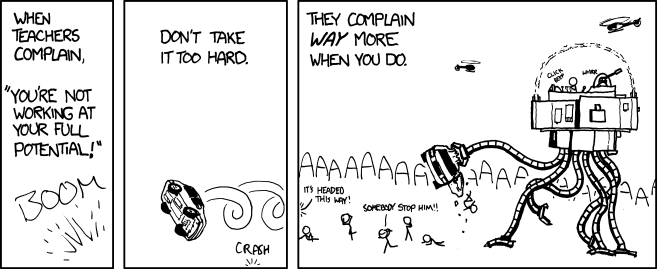
\includegraphics[width=4in]{potential.png}
    \caption*{The bunch of disadvantaged kids I was tutoring became too good at writing, and their essays were forcing me to confront painful existential questions, so I started trying to turn them on to drugs and crime instead.}
\end{figure}

\end{document}
